
%=============================================================================
\section{DDG4 Implementation}
\label{sec:ddg4-user-manual-implementation}
%=============================================================================

\noindent
A basic design criteria of the a \DDG simulation application was to 
process any user defined hook provided by Geant4 as a series of algorithmic
procedures, which could be implemented either using inheritance or by 
a callback mechanism registering functions fulfilling a given signature.
Such sequences are provided for all actions mentioned in the list in 
Section~\ref{sec:ddg4-user-manual-geant4-interface} as well as for 
the callbacks to sensitive detectors.

\noindent
The callback mechanism was introduced to allow for weak coupling between 
the various actions. For example could an action performing monitoring
using histograms at the event level initialize or reset its histograms
at the start/end of each run. To do so, clearly a callback at the 
start/end of a run would be necessary.

\noindent
In the following sections a flexible and extensible interface to hooks
of Geant4 is discussed starting with the description of the basic
components \tts{Geant4Kernel} and \tts{Geant4Action} followed by the 
implementation of the relevant specializations.
The specializations exposed are sequences of such actions,
which also call registered objects.
In later section the configuration and the combination of these components 
forming a functional simulation application is presented.

%=============================================================================
\subsection{The Application Core Object: Geant4Kernel}
\label{sec:ddg4-user-manual-implementation-geant4kernel}
%=============================================================================

\noindent
The kernel object is the central context of a \DDG simulation application and
gives all clients access to the user hooks (see Figure~\ref{fig:ddg4-geant4-kernel}).
All Geant4 callback structures are exposed so that clients can easily 
objects implementing the required interface or register callbacks with the 
correct signature. Each of these action sequences is connected to an instance
of a Geant4 provided callback structure as it is shown in
Figure~\ref{fig:ddg4-g4runmanager-anatomy}.
\begin{figure}[h]
  \begin{center}
    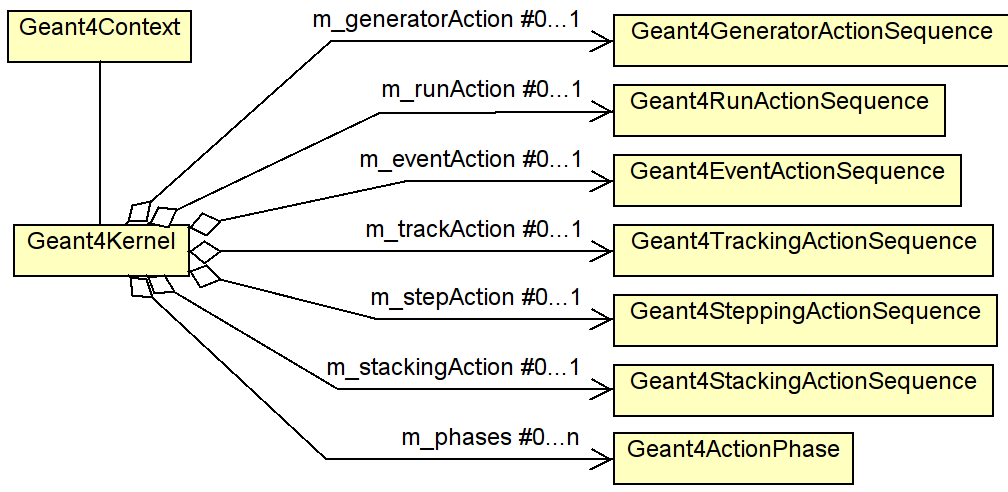
\includegraphics[height=65mm] {DDG4-Geant4Kernel.png}
    \caption{The main application object gives access to all sequencing actions
    in a \DDG4 application. Sequence actions are only container of user actions
    calling one user action after the other. Optionally single callbacks may 
    be registered to a user action.}
    \label{fig:ddg4-geant4-kernel}
  \end{center}
\end{figure}

%=============================================================================
\subsection{Action Sequences}
\label{sec:ddg4-user-manual-implementation-geant4action-sequences}
%=============================================================================

\noindent
As shown in 

%=============================================================================
\subsection{The Base Class of DDG4 Actions: Geant4Action}
\label{sec:ddg4-user-manual-implementation-geant4action-base}
%=============================================================================

\noindent
The class \tts{Geant4Action} is a common component interface providing 
the basic interface to the framework to
\begin{itemize}\itemcompact
\item configure the component using a property mechanism
\item provide an appropriate interface to Geant4 interactivity. The interactivity 
    included a generic way to change and access properties from the Geant4 UI 
    prompt as well as executing registered commands.
\item As shown in Figure~\ref{fig:ddg4-implementation-geant4-action}, the 
    base class also provides to its sub-class a reference to the \tts{Geant4Kernel}
    objects through the \tts{Geant4Context}.
\end{itemize}
The \tts{Geant4Action} is a named entity and can be uniquely identified within
a sequence attached to one Geant4 user callback.
%=============================================================================
\begin{figure}[h]
  \begin{center}
    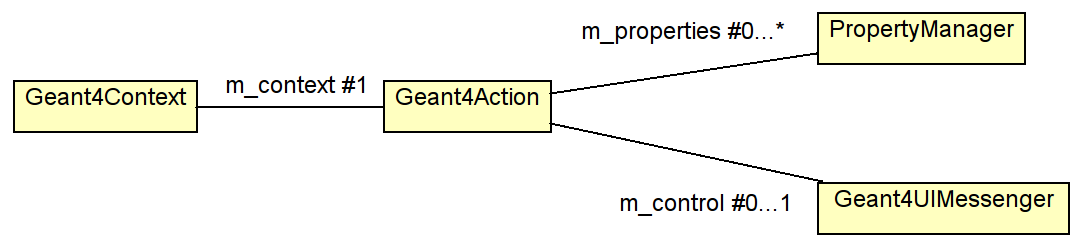
\includegraphics[height=30mm] {DDG4-Geant4Action.png}
    \caption{The design of the common base class \tts{Geant4Action}.}
    \label{fig:ddg4-implementation-geant4-action}
  \end{center}
\end{figure}

\noindent
\DDG knows two types of actions: global actions and anonymous actions.
Global actions are accessible externally from the \tts{Geant4Kernel} instance.
Global actions are also re-usable and hence may be contribute to several 
action sequences (see the following chapters for details). Global actions 
are uniquely identified by their name.
Anonymous actions are known only within one sequence and normally
are not shared between sequences.

%=============================================================================
\subsubsection{The Properties of \bold{Geant4Action} Instances}
\label{sec:ddg4-implementation-geant4-action-properties}
%=============================================================================

\noindent
Nearly any subclass of a \tts{Geant4Action} needs a flexible configuration 
in order to be reused, modified etc. The implementation of the mechanism
uses a very flexible value conversion mechanism using \tts{boost::spirit},
which support also conversions between unrelated types provided a dictionary 
is present.

\noindent
Properties are supposed to be member variables of a given action object.
To publish a property it needs to be declared in the constructor as shown here:
\begin{unnumberedcode}
  declareProperty("OutputLevel", m_outputLevel = INFO);
  declareProperty("Control",     m_needsControl = false);
\end{unnumberedcode}
The internal setup of the \tts{Geant4Action} objects then ensure that 
all declared properties will be set after the object construction to the 
values set in the setup file.

\noindent
\bold{Note:} Because the values can only be set \bold{after} the object 
was constructed, the actual values may not be used in the constructor
of any base or sub-class.

%=============================================================================
\subsection{Geant4 Action Sequences}
\label{sec:ddg4-user-manual-implementation-geant4action-sequences}
%=============================================================================

\noindent
All Geant4 user hooks are realized as action sequences. As shown in 
Figure~\ref{fig:ddg4-geant4-kernel} these sequences are accessible to the user,
who may attach specialized actions to the different action sequences. This 
allows a flexible handing of specialized user actions e.g. to dynamically
add monitoring actions filling histograms or to implement alternative hit 
creation mechanism in a sensitive detector for detailed detector studies.
Figure~\ref{fig:ddg4-implementation-sequence-calls} shows the schematic
call structure of an example {\tt{Geant4TrackingActionSequence}}:\\
\begin{figure}[h]
  \begin{center}
    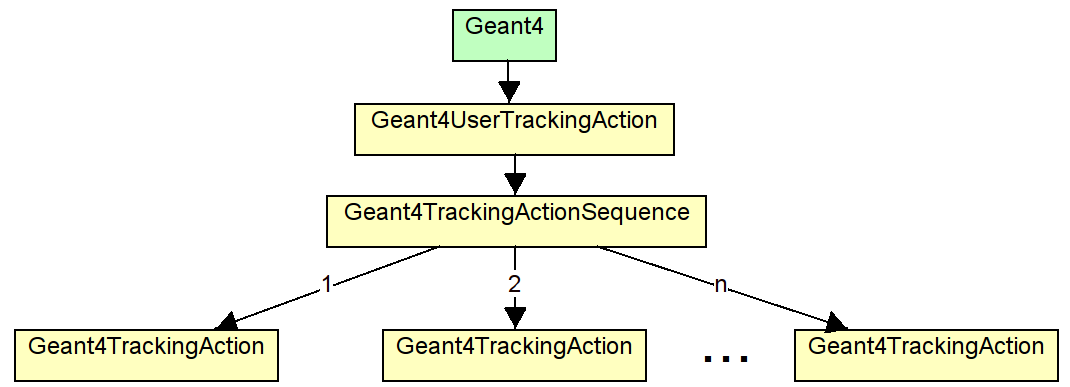
\includegraphics[width=150mm] {DDG4-TrackingActionCalls.png}
    \caption{The design of the tracking action sequence. Specialized 
               tracking action objects inherit from the \tts{Geant4TrackingAction}
               object and must be attached to the sequence.}
    \label{fig:ddg4-implementation-sequence-calls}
  \end{center}
\end{figure}

\noindent
Geant4 calls the function from the virtual interface (\tts{G4UserTrackingAction}), 
which is realised by the \tts{Geant4UserTrackingAction} with the single purpose to
propagate the call to the action sequence, which then calls all registered clients
of type \tts{Geant4TrackingAction}.

\noindent
The main action sequences have a fixed name. These are
\begin{itemize}

\item The \bold{RunAction} attached to the \tts{G4UserRunAction}, implemented 
    by the \tts{Geant4RunActionSequence} class and is called at the start and the end of 
    every run (beamOn). Members of the \tts{Geant4RunActionSequence} are of type
    \tts{Geant4RunAction} and receive the callbacks by overloading the two routines:
\begin{unnumberedcode}
/// begin-of-run callback
virtual void begin(const G4Run* run);
/// End-of-run callback
virtual void end(const G4Run* run);
\end{unnumberedcode}
    or register a callback with the signature {\tts{void (T::*)(const G4Run*)}}
    either to receive begin-of-run or end-or-calls using the methods:
\begin{unnumberedcode}
/// Register begin-of-run callback. Types Q and T must be polymorph!
template <typename Q, typename T> void callAtBegin(Q* p, void (T::*f)(const G4Run*));
/// Register end-of-run callback. Types Q and T must be polymorph!
template <typename Q, typename T> void callAtEnd(Q* p, void (T::*f)(const G4Run*));
\end{unnumberedcode}
    of the \tts{Geant4RunActionSequence} from the \tts{Geant4Context} object.


\item The \bold{EventAction} attached to the \tts{G4UserEventAction}, implemented 
    by the \tts{EventActionSequence} class and is called at the start and the end of 
    every event. Members of the \tts{Geant4EventActionSequence} are of type
    \tts{Geant4EventAction} and receive the callbacks by overloading the two routines:
\begin{unnumberedcode}
/// Begin-of-event callback
virtual void begin(const G4Event* event);
/// End-of-event callback
virtual void end(const G4Event* event);
\end{unnumberedcode}
    or register a callback with the signature {\tts{void (T::*)(const G4Event*)}}
    either to receive begin-of-run or end-or-calls using the methods:
\begin{unnumberedcode}
/// Register begin-of-event callback
template <typename Q, typename T> void callAtBegin(Q* p, void (T::*f)(const G4Event*));
/// Register end-of-event callback
template <typename Q, typename T> void callAtEnd(Q* p, void (T::*f)(const G4Event*));
\end{unnumberedcode}
    of the \tts{Geant4EventActionSequence} from the \tts{Geant4Context} object.


\item The \bold{GeneratorAction} attached to the \tts{G4VUserPrimaryGeneratorAction}, implemented 
    by the \tts{Geant4GeneratorActionSequence} class and is called at the start of 
    every event and provided all initial tracks from the Monte-Carlo generator.
    Members of the \tts{Geant4GeneratorActionSequence} are of type
    \tts{Geant4EventAction} and receive the callbacks by overloading the member function:
\begin{unnumberedcode}
/// Callback to generate primary particles
virtual void operator()(G4Event* event);
\end{unnumberedcode}
    or register a callback with the signature {\tts{void (T::*)(G4Event*)}}
    to receive calls using the method:
\begin{unnumberedcode}
/// Register primary particle generation callback.
template <typename Q, typename T> void call(Q* p, void (T::*f)(G4Event*));
\end{unnumberedcode}
    of the \tts{Geant4GeneratorActionSequence} from the \tts{Geant4Context} object.

\end{itemize}
\begin{figure}[t]
  \begin{center}
    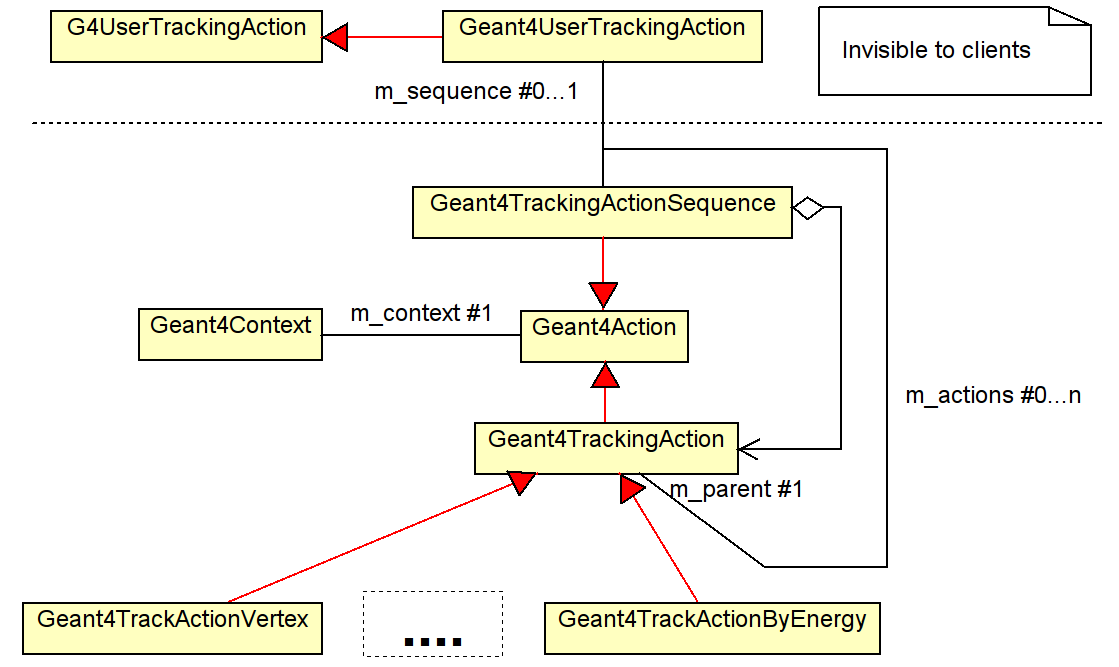
\includegraphics[width=160mm] {DDG4-TrackingAction.png}
    \caption{The design of the tracking action sequence. Specialized 
               tracking action objects inherit from the \tts{Geant4TrackingAction}
               object and must be attached to the sequence.}
    \label{fig:ddg4-implementation-tracking-action}
  \end{center}
\end{figure}

\begin{itemize}
\item The \bold{TrackingAction} attached to the \tts{G4UserTrackingAction}, 
    implemented by the \tts{Geant4-} \tts{Tracking\-Action\-Sequence} class 
    and is called at the start and the end of tracking one single particle 
    trace through the material of the detector.
    Members of the \tts{Geant4\-Tracking\-ActionSequence} are of type
    \tts{Geant4TrackingAction} and receive the callbacks by overloading the member function:
\begin{unnumberedcode}
/// Pre-tracking action callback
virtual void begin(const G4Track* trk);
/// Post-tracking action callback
virtual void end(const G4Track* trk);
\end{unnumberedcode}
    or register a callback with the signature {\tts{void (T::*)(const G4Step*, G4SteppingManager*)}}
    to receive calls using the method:
\begin{unnumberedcode}
/// Register Pre-track action callback
template <typename Q, typename T> void callAtBegin(Q* p, void (T::*f)(const G4Track*));
/// Register Post-track action callback
template <typename Q, typename T> void callAtEnd(Q* p, void (T::*f)(const G4Track*));
\end{unnumberedcode}
Figure~\ref{fig:ddg4-implementation-tracking-action} show as an example 
the design (class-diagram) of the \tts{Geant4TrackingAction}.


\item The \bold{SteppingAction} attached to the \tts{G4UserSteppingAction}, implemented 
    by the \tts{Geant4-} \tts{SteppingActionSequence} class and is called for each
    step when tracking a particle.
    Members of the \tts{Geant4SteppingActionSequence} are of type
    \tts{Geant4SteppingAction} and receive the callbacks by overloading the member function:
\begin{unnumberedcode}
/// User stepping callback
virtual void operator()(const G4Step* step, G4SteppingManager* mgr);
\end{unnumberedcode}
    or register a callback with the signature {\tts{void (T::*)(const G4Step*, G4SteppingManager*)}}
    to receive calls using the method:
\begin{unnumberedcode}
/// Register stepping action callback.
template <typename Q, typename T> void call(Q* p, void (T::*f)(const G4Step*, 
                                                               G4SteppingManager*));
\end{unnumberedcode}


\item The \bold{StackingAction} attached to the 
    {\tts{G4UserStackingAction}}, implemented by the \tts{Geant4-}\\
    \tts{StackingActionSequence} class.
    Members of the \tts{Geant4StackingActionSequence} are of type\\
    \detdesc{html/class_d_d4hep_1_1_simulation_1_1_geant4_stacking_action.html}
    {\tts{Geant4StackingAction}} and receive the callbacks by overloading the member functions:
\begin{unnumberedcode}
/// New-stage callback
virtual void newStage();
/// Preparation callback
virtual void prepare();
\end{unnumberedcode}
    or register a callback with the signature {\tts{void (T::*)()}}
    to receive calls using the method:
\begin{unnumberedcode}
/// Register begin-of-event callback. Types Q and T must be polymorph!
template <typename T> void callAtNewStage(T* p, void (T::*f)());
/// Register end-of-event callback. Types Q and T must be polymorph!
template <typename T> void callAtPrepare(T* p, void (T::*f)());
\end{unnumberedcode}
\end{itemize}

\noindent
All sequence types support the method \tts{void adopt(T* member\_reference)}
to add the members. Once adopted, the sequence takes ownership and manages
the member. The design of all sequences is very similar. 

%=============================================================================
\subsection{Sensitive Detectors}
\label{sec:ddg4-user-manual-geant4sensitivedetectors}
%=============================================================================

\noindent
Sensitive detectors are associated by the detector designers to all active 
materials, which would produce a signal which can be read out. In Geant4 this concept
is realized by using a base class \tts{G4VSensitiveDetector}.
The mandate of a sensitive detector is the construction of hit objects 
using information from steps along a particle track. 
The \tts{G4VSensitiveDetector} receives 
a callback at the begin and the end of the event processing and at each step
inside the active material whenever an energy deposition occurred.

\begin{figure}[t]
  \begin{center}
    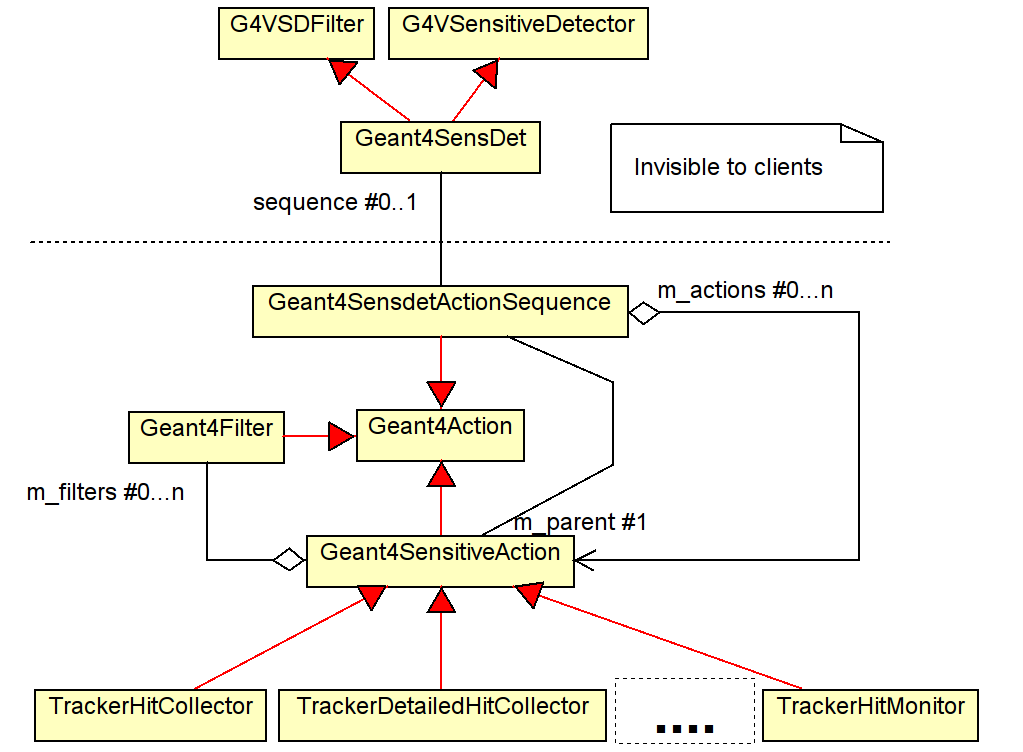
\includegraphics[height=110mm] {DDG4-Sensitive-detector.png}
    \caption{The sensitive detector design. The actual energy deposits are 
        collected in user defined subclasses of the \tts{Geant4Sensitive}.
        Here, as an example possible actions called \tts{TrackerHitCollector},
        \tts{TrackerDetailedHitCollector} and \tts{TrackerHitMonitor} are shown.}
    \label{fig:ddg4-implementation-sensitive-detector}
  \end{center}
\end{figure}

\noindent
The sensitive actions do not necessarily deal only the collection of energy 
deposits, but could also be used to simply monitor the performance of the
active element e.g. by producing histograms of the absolute value or the 
spacial distribution of the depositions.

\noindent
Within \DDG the concept of sensitive  detectors is implemented as a
configurable  action sequence of type 
\detdesc{html/class_d_d4hep_1_1_simulation_1_1_geant4_sens_det_action_sequence.html}
{\tts{Geant4SensDetActionSequence}}
calling members of the type 
\detdesc{html/struct_d_d4hep_1_1_simulation_1_1_geant4_sensitive.html}
{\tts{Geant4Sensitive}} as shown in 
Figure~\ref{fig:ddg4-implementation-sensitive-detector}. The actual processing
part of such a sensitive action is only called if the and of a set of
required filters of type \tts{Geant4Filter} is positive (see also 
section~\ref{sec:ddg4-implementation-sensitive-detector-filters}). No filter 
is also positive. Possible filters are e.g. particle filters, which ignore the
sensitive detector action if the particle is a \tts{geantino} or if the
energy deposit is below a given threshold.

\noindent
Objects of type \tts{Geant4Sensitive} receive the callbacks by overloading the 
member function:
\begin{unnumberedcode}
  /// Method invoked at the beginning of each event.
  virtual void begin(G4HCofThisEvent* hce);
  /// Method invoked at the end of each event.
  virtual void end(G4HCofThisEvent* hce);
  /// Method for generating hit(s) using the information of G4Step object.
  virtual bool process(G4Step* step, G4TouchableHistory* history);
  /// Method invoked if the event was aborted.
  virtual void clear(G4HCofThisEvent* hce);
\end{unnumberedcode}
or register a callback with the signature {\tts{void (T::*)(G4HCofThisEvent*)}}
respectively {\tts{void (T::*)(G4Step*, G4TouchableHistory*)}} 
to receive callbacks using the methods:
\begin{unnumberedcode}
  /// Register begin-of-event callback
  template <typename T> void callAtBegin(T* p, void (T::*f)(G4HCofThisEvent*));
  /// Register end-of-event callback
  template <typename T> void callAtEnd(T* p, void (T::*f)(G4HCofThisEvent*));
  /// Register process-hit callback
  template <typename T> void callAtProcess(T* p, void (T::*f)(G4Step*, G4TouchableHistory*));
  /// Register clear callback
  template <typename T> void callAtClear(T* p, void (T::*f)(G4HCofThisEvent*));
\end{unnumberedcode}
Please refer to the Geant4 Applications manual from the Geant4 web page for 
further details about the concept of sensitive detectors.

%=============================================================================
\subsubsection{Helpers of Sensitive Detectors: The Geant4VolumeManager}
\label{sec:ddg4-user-manual-geant4volumemanager}%=============================================================================

\noindent
Sooner or later, when a hit is created in a sensitive placed volume, the
hit must be associated with this volume. For this purpose \DDhep provides 
the concept of the \tts{VolumeManager}, which identifies placed volumes uniquely 
by a 64-bit identifier, the $CellID$. This mechanism allows to quickly
retrieve a given volume given the hit data containing the $CellID$.
The $CellID$ is a very compressed representation for any element in the 
hierarchy of placed volumes to the sensitive volume in question.

\noindent 
During the simulation the reverse mechanism must be applied: Geant4 provides
the hierarchy of \tts{G4PhysicalVolumes} to the hit location and the local coordinates
of the hit within the sensitive volume. Hence to determine the volume identifier
is essential to store hits so that they can be later accessed and processed efficiently.
This mechanism is provided by the \tts{Geant4VolumeManager}. Clients typically do not
interact with this object, any access necessary is provided by the
\tts{Geant4Sensitive} action:
\begin{unnumberedcode}
  /// Method for generating hit(s) using the information of G4Step object.
  bool MySensitiveAction:process(G4Step* step,G4TouchableHistory* /*hist*/ ) {
    ...
    Hit* hit = new Hit();
    // *** Retrieve the cellID  ***
    hit->cellID = cellID(step);
    ...
  }
\end{unnumberedcode}
The call is realized using a member function provided by the 
\tts{Geant4Sensitive} action:
\begin{unnumberedcode}
  /// Returns the cellID of the sensitive volume corresponding to the step
  /** The CellID is the VolumeID + the local coordinates of the sensitive area.
   *  Calculated by combining the VolIDS of the complete geometry path (Geant4TouchableHistory)
   *  from the current sensitive volume to the world volume
   */
  long long int cellID(G4Step* step);
\end{unnumberedcode}

\noindent
\bold{Note:}\\
The \tts{Geant4VolumeManager} functionality is not for free! It requires that


\noindent
-- match Geant4 volume with TGeo volume

%=============================================================================
\subsubsection{DDG4 Intrinsic Sensitive Detectors}
%=============================================================================
\noindent
Currently there are two generic sensitive detectors implemented in DDG4:
\begin{itemize}\itemcompact
\item The \tts{Geant4TrackerAction}, which may be used to handle tracking devices.
  This sensitive detector produces one hit for every energy deposition of Geant4
  i.e. for every callback to 
\begin{unnumberedcode}
  /// Method for generating hit(s) using the information of G4Step object.
  virtual bool process(G4Step* step, G4TouchableHistory* history);
\end{unnumberedcode}
  See the implementation file 
  \detdesc{html/_geant4_s_d_actions_8cpp_source.html}{DDG4/plugins/Geant4SDAction.cpp}
  for details. The produced hits are of type 
  \detdesc{html/_geant4_data_8h_source.html}{Geant4Tracker::Hit}.

\item The \tts{Geant4CalorimeterAction}, which may be used to handle 
  generic calorimeter like devices.
  This sensitive detector produces at most one hit for every cell in the calorimeter.
  If several tracks contribute to the energy deposit of this cell, the contributions
  are added up.
  See the implementation file 
  \detdesc{html/_geant4_s_d_actions_8cpp_source.html}{DDG4/plugins/Geant4SDAction.cpp}
  for details. The produced hits are of type 
  \detdesc{html/_geant4_data_8h_source.html}{Geant4Calorimeter::Hit}.
  propagate the MC truth information with respect to each track kept in the 
  particle record.
\end{itemize}

\noindent
Both sensitive detectors use the \tts{Geant4VolumeManager} discussed in 
section~\ref{sec:ddg4-user-manual-geant4volumemanager} to identify the sensitive elements.

\noindent
\bold{PLEASE NOTE:}\\
The above palette of generic sensitive detectors only contains two very
often used implementations. We hope, that this palette over time grows from
external contributions of other generic sensitive detectors. We would be happy 
to extend this palette with other generic implementations. One example would
be the handling of the simulation response for optical detectors like RICH-Cerenkov
detectors.

%=============================================================================
\subsubsection{Sensitive Detector Filters}
\label{sec:ddg4-implementation-sensitive-detector-filters}
%=============================================================================

\noindent
The concept of filters allows to build more flexible sensitive detectors by
restricting the hit processing of a given instance of a sensitive action.

\begin{itemize}\itemcompact
\item Examples would be to demand a given particle type before a sensitive action is 
invoked: a sensitive action dealing with optical photons (RICH detectors, etc),
would e.g. not be interested in energy depositions of other particles.
A filter object restricting the particle type to optical photons would 
be appropriate.
\item Another example would be to implement a special action instance, which would
be only called if the filter requires a minimum energy deposit.
\end{itemize}
There are plenty of possible applications, hence we would like 
to introduce this feature here.

\noindent
Filters are called by Geant4 before the
hit processing in the sensitive detectors start. The global filters
may be shared between many sensitive detectors. Alternatively filters
may be directly attached to the sensitive detector in question.
Attributes are directly passed as properties to the filter action.

\noindent
Technically do \tts{Geant4Filter} objects inherit from the base class
\tts{Geant4Filter} (see Figure~\ref{fig:ddg4-implementation-sensitive-detector-filters}.
Any filter inherits from the common base class \tts{Geant4Filter}, then 
several specializations may be configured like filters to select/reject 
particles, to specify the minimal energy deposit to be processed etc.
A sensitive detector is called if the filter callback with the signature
returns a true result:
\begin{unnumberedcode}
  /// Filter action. Return true if hits should be processed
  virtual bool operator()(const G4Step* step) const;
\end{unnumberedcode}
\begin{figure}[h]
  \begin{center}
    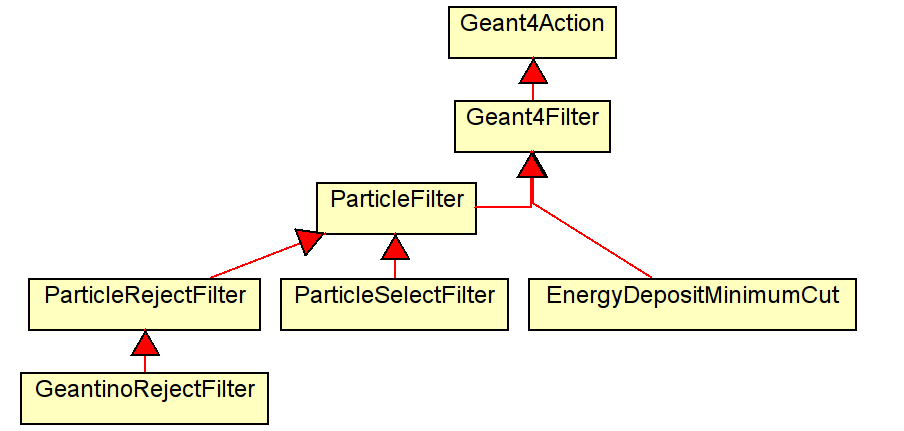
\includegraphics[height=65mm] {DDG4-SensitiveFilterClasses.png}
    \caption{The sensitive detector filters design. The shown class
        diagram is actually implemented.}
    \label{fig:ddg4-implementation-sensitive-detector-filters}
  \end{center}
\end{figure}

\newpage

%=============================================================================
\subsection{The Geant4 Physics List}
\label{sec:ddg4-implementation-physics-list}
%=============================================================================
\noindent 
Geant4 provides the base class \tts{G4VUserPhysicsList}, which allows users
to implement customized physics according to the studies to be made.
Any user defined physics list must provide this interface. DDG4 provides such an interface
through the ROOT plugin mechanism using the class \tts{G4VModularPhysicsList}.
The flexibility of \DDG allows for several possibilities to setup the Geant4
physics list. Instead of explicitly coding the physics list, \DDG foresees the
usage of the plugin mechanism to instantiate the necessary calls to Geant4 in a
sequence of actions:
\begin{itemize}
\item The \bold{physics list} is realized as a sequence of actions of type 
    \detdesc{html/class_d_d4hep_1_1_simulation_1_1_geant4_physics_list_action_sequence.html}
    {\tts{Geant4PhysicsListActionSequence}}.
    Members of the \detdesc{html/class_d_d4hep_1_1_simulation_1_1_geant4_physics_list_action_sequence.html}
    {\tts{Geant4PhysicsListActionSequence}} are of type
    \detdesc{html/class_d_d4hep_1_1_simulation_1_1_geant4_physics_list.html}
    {\tts{Geant4PhysicsList}} and receive the callbacks by overloading 
    the member functions:
\begin{unnumberedcode}
  /// Callback to construct the physics constructors
  virtual void constructProcess(Geant4UserPhysics* interface);
  /// constructParticle callback
  virtual void constructParticles(Geant4UserPhysics* particle);
  /// constructPhysics callback
  virtual void constructPhysics(Geant4UserPhysics* physics);
\end{unnumberedcode}
    or register a callback with the signature {\tts{void (T::*)(Geant4UserPhysics*)}}
    to receive calls using the method:
\begin{unnumberedcode}
  /// Register process construction callback t
  template <typename Q, typename T> void constructProcess(Q* p, void (T::*f)(Geant4UserPhysics*));
  /// Register particle construction callback
  template <typename Q, typename T> void constructParticle(Q* p, void (T::*f)(Geant4UserPhysics*));
\end{unnumberedcode}
    The argument of type \detdesc{html/class_d_d4hep_1_1_simulation_1_1_geant4_user_physics.html}
    {\tts{Geant4UserPhysics}} provides a basic interface to the original
    \tts{G4VModular}- \tts{PhysicsList}, which allows to register physics constructors etc.

\item In most of the cases the above approach is an overkill and often even too flexible.
    Hence, alternatively, the physics list may consist of a single entry of type 
    \detdesc{html/class_d_d4hep_1_1_simulation_1_1_geant4_physics_list.html}
    {\tts{Geant4PhysicsList}}.
\end{itemize}

\noindent
The basic implementation of the \tts{Geant4PhysicsList} supports the usage of various
\begin{itemize}\itemcompact
\item \detdesc{html/_geant4_particles_8cpp_source.html}{particle constructors}, 
    such as single particle constructors like   
    \tts{G4Gamma} or \tts{G4Proton}, or whole particle groups like
    \tts{G4BosonConstructor} or \tts{G4IonConstrutor},
\item \detdesc{html/_geant4_processes_8cpp_source.html}{physics process constructors}, 
    such as e.g. \tts{G4GammaConversion},
    \tts{G4PhotoElectricEffect} or\\ \tts{G4ComptonScattering}, 
\item \detdesc{html/_geant4_physics_constructors_8cpp_source.html}{physics constructors} 
    combining particles and the corresponding 
    interactions, such as\\ e.g. \tts{G4OpticalPhysics},
    \tts{HadronPhysicsLHEP} or \tts{G4HadronElasticPhysics} and
\item \detdesc{html/_geant4_particles_8cpp_source.html}{predefined Geant4 physics lists}, 
    such as \tts{FTFP\_BERT},
    \tts{CHIPS} or \tts{QGSP\_INCLXX}. This option is triggered by the 
    content of the string property "extends" of the \tts{Geant4Kernel::physicsList()} action.
\end{itemize}
These constructors are internally connected to the above callbacks to register themselves. 
The constructors are instantiated using the ROOT plugin mechanism.

\noindent
The description of the above interface is only for completeness. The basic idea is,
that the physics list with its particle and physics constructors is configured
entirely data driven using the setup mechanism described in the following
chapter. However, DDG4 is not limited to the data driven approach. Specialized 
physics lists may be supplied, but there should be no need.
New physics lists could always be composed by actually providing new physics
constructors and actually publishing these using the factory methods:
\begin{code}
// Framework include files
#include "DDG4/Factories.h"

#include "My_Very_Own_Physics_Constructor.h"
DECLARE_GEANT4_PHYSICS(My_Very_Own_Physics_Constructor)
\end{code}
where \tts{My\_Very\_Own\_Physics\_Constructor} represents a sub-class of
\tts{G4VPhysicsConstructor}.

\newpage
%=============================================================================
\subsection{The Support of the Geant4 UI: \tts{Geant4UIMessenger}}
\label{sec:ddg4-user-manual-geant4action-base}
%=============================================================================

\noindent
The support of interactivity in Geant4 is mandatory to debug detector
setups in small steps. The Geant4 toolkit did provide for this reason 
a machinery of UI commands.
\begin{figure}[h]
  \begin{center}
    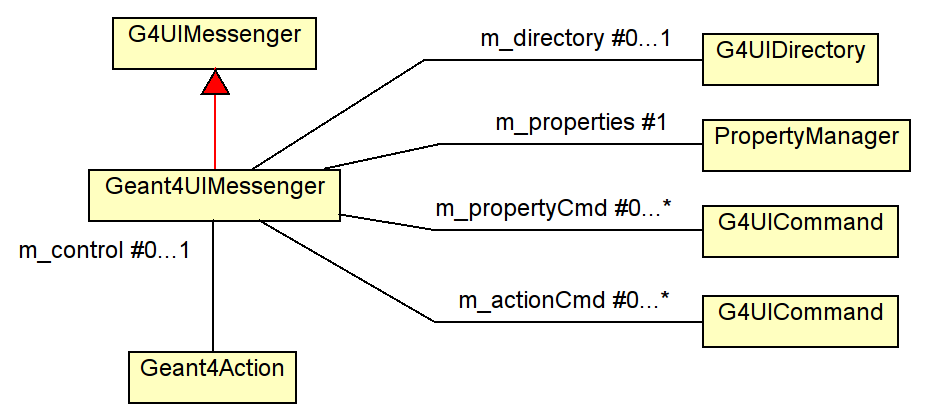
\includegraphics[height=70mm] {DDG4-UIMessenger.png}
    \caption{The design of the \tts{Geant4UIMessenger} class responsible for
        the interaction between the user and the components of \DDG and Geant4.}
    \label{fig:ddg4-tracking-action}
  \end{center}
\end{figure}

\noindent
The UI control is enabled, as soon as the property "Control" (boolean) is set to true.
Be default all properties of the action are exported.
Similar to the callback mechanism described above it is also feasible to
register any object callback invoking a method of a \tts{Geant4Action}-subclass. 

\noindent
The following (shortened) screen dump illustrates the usage of the 
generic interface any Geant4Action offers:
\begin{unnumberedcode}
Idle> ls
Command directory path : /
 Sub-directories : 
   /control/   UI control commands.
   /units/   Available units.
   /process/   Process Table control commands.
   /ddg4/   Control for all named Geant4 actions
   ...
Idle> cd /ddg4
Idle> ls
...
Control for all named Geant4 actions

 Sub-directories : 
   /ddg4/RunInit/   Control hierarchy for Geant4 action:RunInit
   /ddg4/RunAction/   Control hierarchy for Geant4 action:RunAction
   /ddg4/EventAction/   Control hierarchy for Geant4 action:EventAction
   /ddg4/GeneratorAction/   Control hierarchy for Geant4 action:GeneratorAction
   /ddg4/LCIO1/   Control hierarchy for Geant4 action:LCIO1
   /ddg4/Smear1/   Control hierarchy for Geant4 action:Smear1
   /ddg4/PrimaryHandler/   Control hierarchy for Geant4 action:PrimaryHandler
   /ddg4/TrackingAction/   Control hierarchy for Geant4 action:TrackingAction
   /ddg4/SteppingAction/   Control hierarchy for Geant4 action:SteppingAction
   /ddg4/ParticleHandler/   Control hierarchy for Geant4 action:ParticleHandler
   /ddg4/UserParticleHandler/   Control hierarchy for Geant4 action:UserParticleHandler
   ...
Idle> ls Smear1
Command directory path : /ddg4/Smear1/
 ...
 Commands : 
   show * Show all properties of Geant4 component:Smear1
   Control * Property item of type bool
   Mask * Property item of type int
   Name * Property item of type std::string
   Offset * Property item of type ROOT::Math::LorentzVector<ROOT::Math::PxPyPzE4D<double> >
   OutputLevel * Property item of type int
   Sigma * Property item of type ROOT::Math::LorentzVector<ROOT::Math::PxPyPzE4D<double> >
   name * Property item of type std::string
Idle> Smear1/show
PropertyManager: Property Control = True
PropertyManager: Property Mask = 1
PropertyManager: Property Name = 'Smear1'
PropertyManager: Property Offset = ( -20 , -10 , -10 , 0 )
PropertyManager: Property OutputLevel = 4
PropertyManager: Property Sigma = ( 12 , 8 , 8 , 0 )
PropertyManager: Property name = 'Smear1'

Idle> Smear1/Offset (200*mm, -3*mm, 15*mm, 10*ns)
Geant4UIMessenger: +++ Smear1> Setting property value Offset = (200*mm, -3*mm, 15*mm, 10*ns)  
                               native:( 200 , -3 , 15 , 10 ).
Idle> Smear1/show                                
...
PropertyManager: Property Offset = ( 200 , -3 , 15 , 10 )

\end{unnumberedcode}

\newpage
